\documentclass[]{exam}
\usepackage{epic,array,ecltree,url,calrsfs}
\usepackage[nointegrals]{wasysym}

%These tell TeX which packages to use.
\usepackage{array,epsfig}
\usepackage{amsmath}
\usepackage{amsfonts}
\usepackage{amssymb}
\usepackage{amsxtra}
\usepackage{amsthm}
\usepackage{mlextra} % must come after ams packages
\usepackage{mathrsfs}
\usepackage[dvipsnames]{xcolor}
\usepackage{array}
\usepackage{graphicx}
\graphicspath{ {../art/} }
\usepackage{bm}
\usepackage{tikz}
\usepackage{multicol}
\usepackage{enumitem}

\newcommand{\twonode}{%
  \begingroup\normalfont
  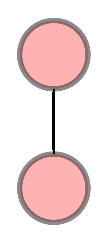
\includegraphics[height=\fontcharht\font`\b]{2nodetree.eps}%
  \endgroup
}


\title{Lab 6: Clausal Form, Resolution}
\author{Foundations of Computer Science}
\date{\today}
%\pagestyle{empty} 
%\footer{}{\thepage}{}
\unframedsolutions
\SolutionEmphasis{\itshape\small}
\SolutionEmphasis{\color{NavyBlue}}


\begin{document}

\maketitle

\setlength{\columnseprule}{1pt}
\begin{questions} 

\question Consider the following circuit:
\begin{center}
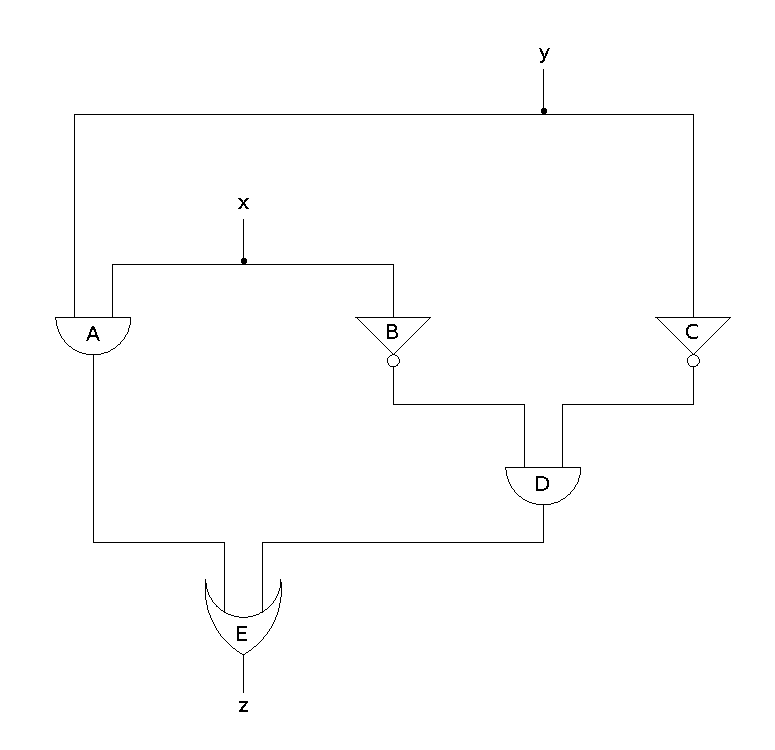
\includegraphics[height=8cm]{equiv_circuit.eps}%
\end{center}

\begin{parts}
\part Write a statement in propositional logic that expresses
$z$ in terms of $x$ and $y$.
\begin{solution}
$z \eqv (x\land y) \lor \ngg (x \land y)$
\end{solution}

\part What logical operator does this circuit implement?
\begin{solution}
$\eqv$
\end{solution}
\end{parts}

\question Transform the set of formulas below into clausal form and refute 
          using resolution.
\[
  \{p,\: p\imp ((q\lor r) \land \ngg (q \land r)),\: p \imp ((s \lor t) \land
      \ngg (s \land t)),\:  s \imp q,\: \ngg r \imp t,\: t \imp s \}
  \]
\begin{solution}
Proceed by changing all formulas to their corresponding CNF. The first formula
is trivial. The second can be converted as follows:
\begin{align*}
&p \imp ((q\lor r) \land \ngg (q \land r))                            && \text{original} & \\
&\equiv \ngg p\lor ((q\lor r) \land \ngg (q \land r))                 && A\imp B \equiv \ngg A \lor B &\\ 
&\equiv \ngg p\lor ((q\lor r) \land (\ngg q \lor \ngg r))             && \text{De Morgan's Laws} &\\  
&\equiv (\ngg p\lor (q\lor r)) \land (\ngg p\lor (\ngg q \lor \ngg r))&& A \lor (B \land C) \equiv (A \lor B) \land (B \lor C)&\\ 
&\equiv (\ngg p\lor q\lor r) \land (\ngg p \lor \ngg q \lor \ngg r)   && \text{associative property} &\\   
&\equiv \{\bar{p}qr, \bar{p}\bar{q}\bar{r} \}                         && \text{clausal form}&\\ 
\end{align*}
The third formula has the same form with different variables, so by the same transformations:
\begin{align*}
&p \imp ((s \lor t) \land \ngg (s \land t)) \\ 
&\equiv \{\bar{p}st, \bar{p}\bar{s}\bar{t} \} \\ 
\end{align*}
The rest of the formulas follow immediately from simple transformations.
Putting these all together in a single set, we have

\[
  \{p, \bar{p}qr, \bar{p}\bar{q}\bar{r}, \bar{p}st, \bar{p}\bar{s}\bar{t}, \bar{s}q, rt, \bar{t}s\}
\]
~\\{ \bf One possible refutation:}
\begin{enumerate}
\item $p,\bar{p}st$: $st$
\item $st,\bar{t}s$: $s$
\item $p,\bar{p}\bar{s}\bar{t}$: $\bar{s}\bar{t}$
\item $s,\bar{s}\bar{t}$: $\bar{t}$
\item $s,\bar{s}q$: $q$
\item $p,\bar{p}\bar{q}\bar{r}$: $\bar{q}\bar{r}$
\item $q,\bar{q}\bar{r}$: $\bar{r}$
\item $\bar{r}, rt$: $t$
\item $t,\bar{t}$: $\Box$
\end{enumerate}

\end{solution}
\question Refer to the following diagram of a half-adder circuit and
answer the questions below: 
\begin{center}
\begin{picture}(280,120)
\put(-10,  0){\makebox(20,20)[l]{Bit2}}
\put(-10,100){\makebox(20,20)[l]{Bit1}}
\put(260, 20){\makebox(25,20)[l]{Sum}}
\put(260, 90){\makebox(25,20)[l]{Carry}}
\put(20, 10){\line(1,0){60}}
\put(20,110){\line(1,0){50}}
\put(30, 10){\line(1,2){40}}
\put(30,110){\line(1,-2){40}}
\put(70, 30){\line(1,0){10}}
\put(70,80){ %AND gate
  \put(20,20){\oval(40,40)[r]}
  \put(0,0){\line(0,1){40}}
  \put(0,0){\line(1,0){20}}
  \put(0,40){\line(1,0){20}}
}
\put(70,0){ %OR gate
  \put(20,20){\oval(40,40)[r]}
  \put(0,20){\oval(20,40)[r]}
  \put(0,0){\line(1,0){20}}
  \put(0,40){\line(1,0){20}}
}
\put(110,100){\line(1,0){140}}
\put(110, 20){\line(1,0){60}}
\put(210, 30){\line(1,0){40}}
\put(170,10){ %AND gate
  \put(20,20){\oval(40,40)[r]}
  \put(0,0){\line(0,1){40}}
  \put(0,0){\line(1,0){20}}
  \put(0,40){\line(1,0){20}}
}
\put(130,80){  % NOT gate
  \put( 0, 0){\line(1,0){20}}
  \put( 0, 0){\line(1,-2){10}}
  \put(20, 0){\line(-1,-2){10}}
  \put(10,-23){\circle{6}}
}
\put(140,80){\line(0,1){20}}
\put(140,54){\line(0,-1){14}}
\put(140,40){\line(1,0){30}}
\end{picture}
\end{center}

(Note: In the questions below the variables $b_1$,$b_2$, $c$ and $s$ refer to
``Bit1'', ``Bit2'', ``Carry'', and ``Sum'', respectively, in the above
diagram.)
\begin{parts}
\part Write a formula in propositional logic that expresses the relationship
between $b_1$, $b_2$ and $c$. The formula should be true when the
values of the three variables correspond to the expected behavior of the
circuit, and false otherwise.
\begin{solution}
$c \eqv b_1 \land b_2$
\end{solution}

\part Write a formula in propositional logic that expresses the relationship
between $b1$, $b2$ and $s$.
\begin{solution}
$s \eqv \ngg(b1 \land b2) \land (b1 \lor b2)$
\end{solution}
\part Transform the formulas to a set of clauses.
\begin{solution}
$\{\bar{s}\bar{b1}\bar{b2}, \bar{s}b1b2, s\bar{b1}b2, sb1\bar{b2}, \bar{c}b1, \bar{c}b2, c\bar{b1}\bar{b2}\}$
\end{solution}

\part\label{q:addunsat} Show that the addition of the unit clauses $\{b1,b2,\bar{s},\bar{c}\}$
gives an unsatisfiable set.
\begin{solution}
$\{\bar{s}\bar{b1}\bar{b2}, \bar{s}b1b2, s\bar{b1}b2, sb1\bar{b2}, \bar{c}b1,
  \bar{c}b2, c\bar{b1}\bar{b2},b1,b2,\bar{s},\bar{c}\}$
\begin{enumerate}
\item $c\bar{b1}\bar{b2}, \bar{c}$: $\bar{b1}\bar{b2}$ 
\item $\bar{b1}\bar{b2}, b1$: $\bar{b2}$ 
\item $\bar{b2}, b2$: $\Box$ 
\end{enumerate}
\end{solution}

\part\label{q:addsat} Show that the addition of the unit clauses $\{b1,b2,\bar{s},c\}$
gives satisfiable set.
\begin{solution}
In order for the set to be satisfiable, all the unit clauses must evaluate to
$T$. There is only one interpretation, $\mathcal{I}$, that meets this criteria: it is defined
by $\mathcal{I}(b1) = \mathcal{I}(b2) = \mathcal{I}(c) = T$ and $\mathcal{I}(s)
  = F$. Observe that under this interpretation, there is at least one literal
with the value of $T$ in every clauses, so all clauses evaluate to $T$.
\end{solution}

\part Explain what your answers to (\ref{q:addunsat}) and (\ref{q:addsat})  means in terms 
of the behavior of the circuit.
\begin{solution}
The clauses that give an unsatisfiable set force an interpretation that
corresponds to $1+1 = 0$ carry $0$, which is incorrect behavior for this
circuit. The unit clauses that result in a satisfiable set correspond to
the interpretation $1+1 = 0$ carry $1$, which is correct.
\end{solution}
\end{parts}

\end{questions}
\end{document}


